\section{Results on the real engines}\label{sec:results}

\subsection{The thrashing curve at two pool sizes}\label{sec:curve}

\begin{figure*}[t]
\centering
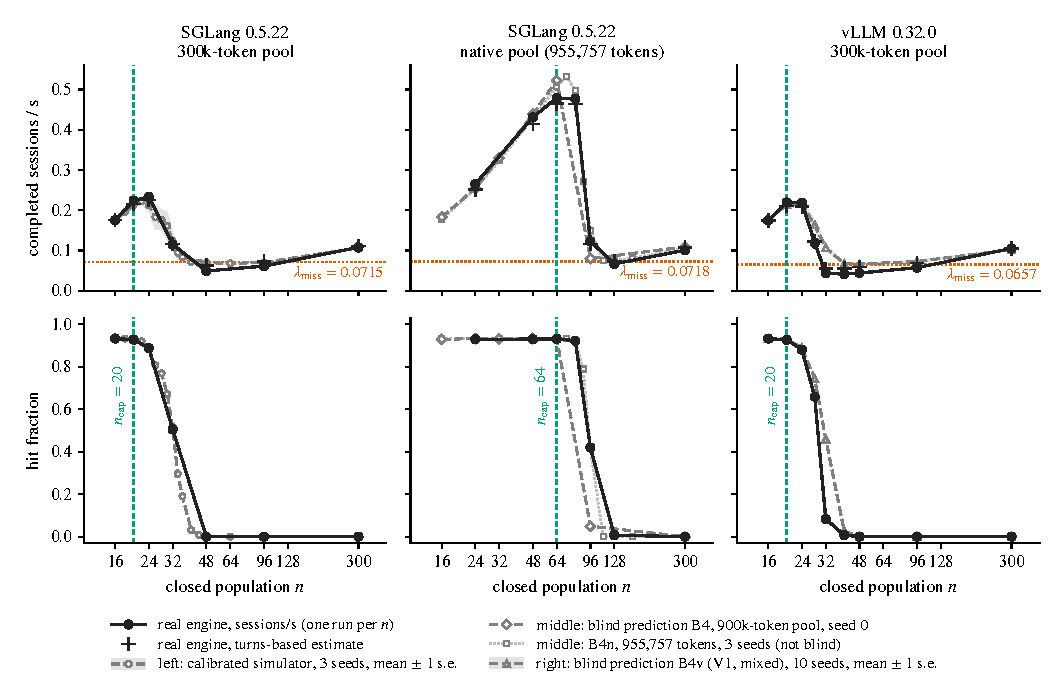
\includegraphics[width=0.92\textwidth]{figs/fig2_thrashing_curve.pdf}
\caption{Closed-population thrashing curve, real engine (black, filled; one run per $n$) against the simulator (gray, open, dashed). Top: $\mu(n)$ in completed sessions/s (plus signs: turns-based estimate); bottom: hit fraction. Left: SGLang, 300k-token pool; calibrated simulator, mean of 3 seeds $\pm$1 s.e. Middle: SGLang, native pool (955,757 tokens); blind prediction B4 at 900k tokens (seed 0); light gray, dotted: B4n at the real pool (3-seed mean), which is not blind (\S\ref{sec:blind}). Right: vLLM 0.32.0, 300k-token pool; blind prediction B4v (variant V1: token costs scaled to vLLM's all-miss rate; mixed batching), mean of 10 seeds $\pm$1 s.e. (\S\ref{sec:vllm}). Dotted: each cell's $\lmiss$. Green dashed: the registered caps, $n=20$, 64 and 20.}\label{fig:curve}
\end{figure*}

With the 300k pool (Fig.~\ref{fig:curve}, left), $\mu(n)$ rises from 0.176\sps{} at $n=16$ to 0.224 at 20 and 0.233 at 24, with hit fractions 0.93, 0.93 and 0.89. The run at $n=24$, which sets $\mu^*$, contains a degraded episode inside its window (hit fraction 0.66 over $[900,1200)$\,s, 0.46 in its worst 100\,s); over $[1200,2700)$\,s alone $\mu(24)=0.257$ against $\mu(20)=0.231$, so the near-tie that sets the cap of 20 owes part of its closeness to this episode. The run at $n=32$ mixes two regimes: degraded from about 450 to 2400\,s, then recovered to 0.80, for a hit fraction of 0.51. At $n=48$ none of the 20.0M prompt tokens in the window was served from cache: evictable tokens survive about 6.3\,s before eviction (estimated as mean evictable KV over the eviction rate) while a session returns after 30.6\,s on average (2.9\,s against 66\,s at $n=96$). The cliff is where memory predicts ($\Nlb\approx28.5$; the hit fraction crosses 0.5 at $n=32.2$), just below the all-miss onset $n_b=32.7$ of the first-principles model, which predicts this curve without using its points (\S\ref{sec:fp}, Table~\ref{tab:fpval}). Token-level hit rates have been reported to collapse as concurrent agents grow on SGLang~\citep{chen2026concur} and on vLLM~\citep{yuan2026agentic,hong2026misat}; what we add is $\mu(n)$ in completed sessions per second, the quantity the open-system model uses, at two pool sizes and, in \S\ref{sec:vllm}, on a second engine. Beyond the peak the curve is not monotone: it falls to $\mu(48)=0.049$\sps{} and rises again, $\mu(96)=0.061<\mu(300)=0.108$\sps. We attribute both to the synchronized start, which leaves old, long turns in the window at $n=48$ (served prompts 14\% above the stationary mean) and young sessions with short prompts at $n=300$ (71\% of the stationary length in flight); no longer run has tested this; the all-miss level implied by token throughput is roughly flat at 0.072--0.081\sps, so the collapse from the peak is about threefold. Stock LPM keeps 39\% of turns hitting at $n=48$ (rising from 0.28 to 0.44 through the window); at $n=300$ its queue of 269 exceeds the 128-request threshold above which, by the source, SGLang's LPM stops re-sorting its queue, and no turn hits; whether the fallback causes the zero was not tested (at $n=300$ the pool may be oversubscribed under any ordering).

With the native pool (Fig.~\ref{fig:curve}, middle), SGLang sized the KV pool at 955,757 tokens, 3.19 times the 300k pool. $\mu$ peaks at 0.479\sps{} at $n=64$ (0.477 at 80) with 92--93\% of turns hitting, then falls to 0.123 at $n=96$ (hit fraction 0.42), 0.067 at 128 (0.007) and 0.101 at 300. The hit fraction crosses 0.5 between $n=80$ (0.92) and 96 (0.42), near 93 by linear interpolation, against just above 32 at 300k; the peak is at 64--80 against 20--24. With one run per $n$, the cliff moves out roughly threefold. The all-miss capacity is unchanged within its standard error: $0.0718\pm0.0037$\sps{} turns-based against $0.0715\pm0.0038$, and $11{,}282\pm51$ against $11{,}243\pm84$ all-miss tokens/s. The 300k-token pool limit did not create the cliff; it moved it. The ratio $\mu^*/\lref$ is 6.67 with the native pool and 3.26 at 300k.\footnote{These are the registered values: the peak in completed sessions over the turns-based $\lref$. Turns-based over turns-based gives 6.48 and 3.15.}

\subsection{The all-miss capacity and the from-empty edge}\label{sec:edge}
E0a gives $\lref=0.0715\pm0.0038$\sps{} turns-based (standard error over three seeds), our estimate of $\lmiss$, $0.0717\pm0.0076$ in completed sessions, and $11{,}243\pm84$ all-miss prefill tokens/s. The token rate varies by $\pm1.2\%$ across seeds and the session rate by $\pm17\%$: the engine is bound by prefill tokens, and the sessions completed in 1800\,s are a small sample of a heavy-tailed quantity. The token rate divided by $E[W]$ gives 0.0728\sps, within 2\% of the turns-based value.

\begin{figure}[t]
\centering
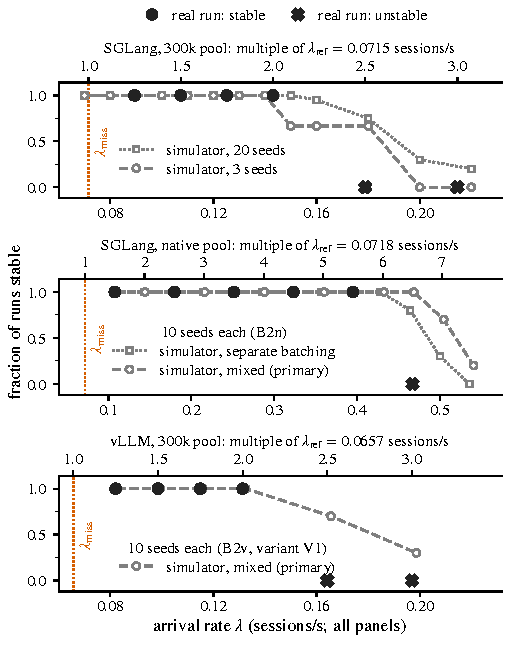
\includegraphics[width=\columnwidth]{figs/fig3_from_empty_stability.pdf}
\caption{From-empty stability. Real engine: one 3000\,s run per rate from an empty cache and queue (1 = stable, 0 = unstable), plotted at its nominal rate; all runs used arrival seed 0, whose realized rates were 6--13\% higher. Gray: blind simulator predictions, the fraction of simulated runs stable at multiples of the simulator's own $\lmiss$. Top, SGLang with the 300k pool: B2 (3 seeds dashed, 20 dotted). Middle, SGLang with the native pool: B2n (10 seeds; mixed batching, the primary mode, dashed; separate, dotted). Bottom, vLLM 0.32.0 with the 300k pool: B2v (variant V1, costs scaled to vLLM; mixed batching, 10 seeds). Top axes: multiples of each cell's $\lref$ (the simulators' own $\lmiss$ are 0.0722 at 300k, 0.0720 and 0.0714 native, and 0.0662 for B2v).}\label{fig:edge}
\end{figure}

From an empty cache and queue (Fig.~\ref{fig:edge}, top) the engine stayed stable at 1.25, 1.5, 1.75 and 2.0 $\lref$, ending each run with an empty queue and with 91--93\% of turns hitting over the run, and was unstable at 2.5 $\lref$ (final queue 127, rising by 146 over the last 1500\,s) and 3.0 (289 and 196). The edge lies between 2.0 and 2.5 $\lref$, well below $\mu^*/\lref=3.26$, so the from-empty edge, not the peak, bounds the window. The registered window was $(1,\,2.0)\,\lref=(0.0715,\,0.143)$\sps. Each rate is one 3000\,s run; a longer horizon could find a lower edge, and at 2.0 $\lref$ the hit fraction fell from 0.934 in $[300,1500)$\,s to 0.903 in the second half of the run. All six runs used seed 0, so they share one random-number stream: their arrival sequences are nested, and each arrival count lies about 2.1 standard deviations above its Poisson mean, 8--13\% above the nominal rate (302, 359, 416, 472, 585 and 697 sessions; the runs labelled 2.0 and 2.5 $\lref$ received 2.20 and 2.73 $\lref$). This makes the stable side of the bracket conservative and its unstable side weaker than the labels suggest; in realized arrivals the bracket is still below $\mu^*/\lref$.

With the native pool (Fig.~\ref{fig:edge}, middle; native E0b, rates in multiples of the native $\lref=0.0718$\sps) the engine stayed stable at 1.5, 2.5, 3.5, 4.5 and 5.5 $\lref$, ending each run with an empty queue and with 93\% of turns hitting over the run, and was unstable at 6.5 $\lref$: its final queue was 505, rising by 477 over the last 1500\,s, and its hit fraction fell from 0.84 in $[300,1500)$\,s to 0.00 in the second half. In nominal rates the edge lies between 5.5 and 6.5 $\lref$ (0.395 and 0.467\sps), so the native window is $(1,\,5.5)\,\lref$. Unlike at 300k, this does not show the edge below the peak ($\mu^*/\lref=6.67$, or 6.48 turns-based): these runs also used seed 0 (361 to 1478 sessions, 5.6--11.7\% above nominal), and the 6.5 run received 0.493\sps{} (6.86 $\lref$), above the measured peak, so overload alone can explain its instability. The stable 5.5 run received 0.419\sps{} (5.84 $\lref$). Its upper edge is 2.75 times higher than at 300k in units of $\lref$ (5.5 against 2.0), and the window is $4.5\,\lref$ wide against $1.0$. Again each rate is a single 3000\,s run.

\subsection{The registered paired test}\label{sec:e2}

\begin{table}[t]
\centering\footnotesize
\caption{The three registered tests: the two pre-registered SGLang tests, E2 (300k-token pool, cap 20, $\lref=0.0715$\sps) and native E2 (955,757-token pool, cap 64, $\lref=0.0718$\sps), and the registered vLLM test (300k-token pool, cap 20, $\lref=0.0657$\sps). States for seeds 0, 1, 2: T trapped, I indeterminate, D draining, G good, R recovered. Hit fraction, uncached prefill rate in multiples of the all-miss rate, mean backlog (sessions in the system) and its slope (sessions/s) over the evaluation window; ranges over seeds; good-arm slopes in absolute value. Slope thresholds: 0.0125, 0.0232, 0.0538 and 0.1077 at 1.35, 1.65, 2.5 and 4.0 $\lref$ on SGLang, 0.0115 and 0.0213 at 1.35 and 1.65 $\lref$ on vLLM. Rates are nominal; the base arrivals realized in the window, which the three arms of a seed share, were 1.45, 1.27, 1.42; 1.73, 1.61, 1.75; 2.73, 2.48, 2.58; 4.28, 3.89, 4.09; and on vLLM 1.45, 1.24, 1.41 and 1.76, 1.56, 1.74 $\lref$ for seeds 0, 1, 2.}\label{tab:e2}
\setlength{\tabcolsep}{3pt}
\resizebox{\columnwidth}{!}{%
\begin{tabular}{@{}c l c c c c c@{}}
\toprule
$\lambda/\lref$ & arm & states & hit & tokens & backlog & slope\\
\midrule
\multicolumn{7}{@{}l}{\emph{300k-token pool (E2)}}\\
1.35 & BURST   & T I T & 0.000 & 1.009--1.025 & 200--232 & 0.0036--0.0222\\
     & NOBURST & G G G & 0.930--0.934 & 0.08--0.09 & 7.9--9.7 & ${<}0.001$\\
     & CAPPED  & R R R & 0.930--0.934 & 0.08--0.09 & 7.9--9.7 & ${<}0.001$\\
\addlinespace
1.65 & BURST   & T T T & 0.000 & 1.025--1.029 & 283--332 & 0.0277--0.0362\\
     & NOBURST & G G G & 0.921--0.934 & 0.10--0.13 & 10.9--11.8 & ${<}0.002$\\
     & CAPPED  & R R R & 0.929--0.934 & 0.10--0.11 & 10.9--11.7 & ${<}0.002$\\
\midrule
\multicolumn{7}{@{}l}{\emph{native pool (native E2)}}\\
2.5  & BURST   & T T T & 0.000 & 1.074--1.078 & 557--601 & 0.079--0.085\\
     & NOBURST & G G G & 0.929--0.935 & 0.15--0.16 & 15.6--18.5 & ${<}0.003$\\
     & CAPPED  & R R R & 0.929--0.935 & 0.15--0.16 & 15.6--18.5 & ${<}0.003$\\
\addlinespace
4.0  & BURST   & T T T & 0.000 & 1.106--1.124 & 1098--1139 & 0.146--0.164\\
     & NOBURST & G G G & 0.929--0.935 & 0.24--0.27 & 28.2--33.6 & ${<}0.004$\\
     & CAPPED  & R R R & 0.929--0.935 & 0.24--0.27 & 28.1--33.5 & ${<}0.004$\\
\midrule
\multicolumn{7}{@{}l}{\emph{vLLM 0.32.0, 300k-token pool (registered, not pre-registered)}}\\
1.35 & BURST   & T D T & 0.000 & 0.995--1.012 & 201--222 & $-5\times10^{-5}$--0.0170\\
     & NOBURST & G G G & 0.930--0.931 & 0.07--0.09 & 7.0--8.4 & ${<}0.001$\\
     & CAPPED  & R R R & 0.930--0.931 & 0.07--0.09 & 7.0--8.4 & ${<}0.001$\\
\addlinespace
1.65 & BURST   & T I T & 0.000 & 0.948--1.018 & 281--330 & 0.0183--0.0341\\
     & NOBURST & G G G & 0.932--0.933 & 0.10--0.11 & 9.3--10.8 & ${<}0.001$\\
     & CAPPED  & R R R & 0.932--0.933 & 0.10--0.11 & 9.3--10.9 & ${<}0.001$\\
\bottomrule
\end{tabular}}
\end{table}

The registered analysis, run on all 18 runs with the code frozen at the registration commit, passes at both rates (Table~\ref{tab:e2}, top); by the definition of \S\ref{sec:prereg} the test is pre-registered. Every BURST run had a hit fraction of 0.000 over the evaluation window, an uncached prefill rate of 1.009--1.029 times the all-miss rate and a mean backlog of 200--332 sessions. One (1.35 $\lref$, seed 1) is stuck in the same way, but its backlog was flat over the window (207 sessions at its start, 206 at its end; slope 0.0036\sps, below the 0.0125 threshold), so the rule calls it indeterminate: its seed delivered 0.0910 arrivals/s in the window, 5.8\% below the nominal 0.0966 (seeds 0 and 2: 0.1037 and 0.1017), and the trapped engine completed 0.0913\sps. The pass at 1.35 $\lref$ therefore rests on 2 of 3 seeds, the minimum the rule allows. The other runs' base arrivals over the window came to 1.42 and 1.45 $\lref$ at 1.35 and 1.61--1.75 $\lref$ at 1.65 (Table~\ref{tab:e2}). Every NOBURST and CAPPED run is good (hit fractions 0.921--0.934, backlogs of 8--12 sessions, most asleep in tool calls); in the window CAPPED cannot be told apart from NOBURST, because the gate had drained the burst. The counts are small, and pooling the two rates does not make them independent: both rates use the same three seeds, with the same burst and nested arrivals (\S\ref{sec:harness}). BURST's hit fraction is below NOBURST's in all six seed-and-rate pairs; counting each seed once, a post-hoc one-sided sign test gives $p=1/8$, the smallest value three seeds allow.

In Fig.~\ref{fig:e2}, every BURST run is at zero hits from the window starting at 1300\,s to the end. Its backlog first fell, to 135--172 sessions 300--1300\,s after the burst, as short burst sessions finished, then rose; over the last 300\,s it was 206--369 sessions, still growing in five runs and flat in the sixth. The five trapped runs still completed 0.081--0.097\sps{} (1.13--1.35 $\lref$), above $\lmiss$, because the backlog's sessions are young and their turns short, so that at about the all-miss token rate more turns, and more sessions, complete (\S\ref{sec:fluid}), but below the arrival rate, and the sixth completed sessions about as fast as they arrived (1.28 and 1.27 $\lref$); only the uncached prefill rate sits at the all-miss level, which is why the registered rule uses tokens. The CAPPED gate's queue emptied 1547--1904\,s after the burst at 1.35 $\lref$ and 2021--2693\,s at 1.65 $\lref$, 3--52\% longer than the fluid estimate of \S\ref{sec:props} from the population present at the burst (1453--1508\,s and 1757--1804\,s; the registration's cruder estimate was 1571\,s and 1889\,s), and well before the evaluation window. Outside the registered criteria, the CAPPED arm's hit fraction dips while the gate drains the burst: its lowest 100\,s window is 0.48--0.77 in four of six runs, against 0.82--0.89 for NOBURST, which plausibly slowed the drain. The cap has a cost that the registered criteria do not measure: it turns the burst into admission delay at the client. In each CAPPED run 349--543 sessions waited at the gate, 45--66\% of them ordinary arrivals queued behind the burst, for 405--471\,s on average and at most 853--985\,s; outside the drain the gate bound only briefly, when arrivals clustered (at most 40 sessions in a run, each for less than 50\,s). Without the cap, turns completed in the BURST arm's evaluation window took a mean of 163--237\,s from send to completion (the client does not stream), against 1.4--1.7\,s in NOBURST and CAPPED and 1.4--1.5\,s in every arm before the burst; at 8700\,s, 19--29\% of BURST sessions were unfinished. So at loads that the engine carried from empty for the full 8700\,s run (E0b carried the bracketing rates, 1.25--1.75 $\lref$, for 3000\,s), 200 sessions arriving within a minute, an order of magnitude more than the 8--12 present in the good state, moved it into an all-miss state that it did not leave within 7500\,s, and a cap of 20 sessions, within 5\% of the measured peak of $\mu(n)$ (argmax $n=24$), prevented that at the price of that admission delay. The heuristic F2 of \S\ref{sec:fp} puts the probability that a run at these rates leaves the good state on its own within 8700\,s at about 0.5\% at 1.35 and 5\% at 1.65 $\lref$, so good NOBURST arms over 8700\,s are the expected outcome, not evidence that the good state never ends.

\subsection{The registered test with the native pool}\label{sec:e2native}

\begin{figure*}[t]
\centering
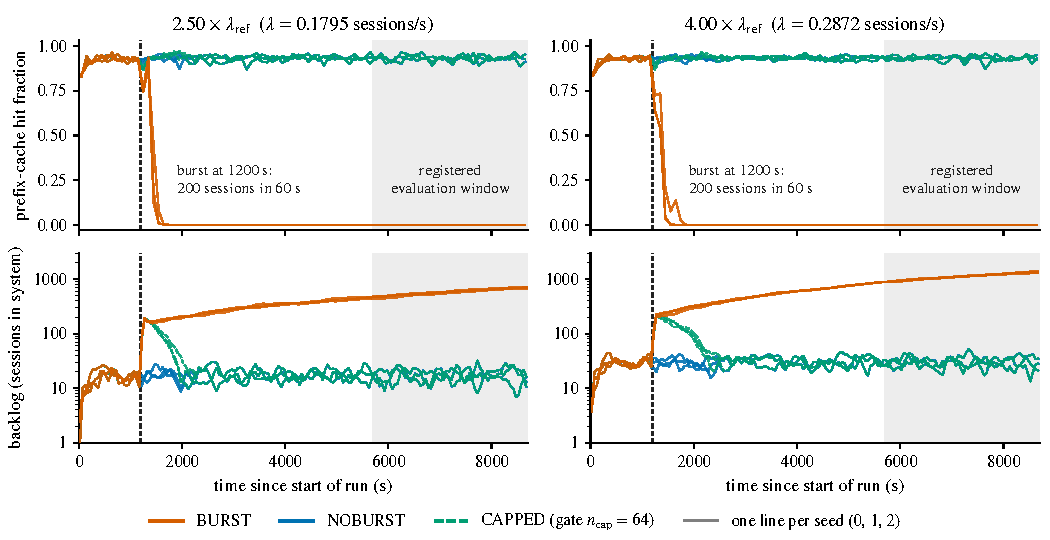
\includegraphics[width=\textwidth]{figs/fig7_e2_native_timeseries.pdf}
\caption{The registered test with the native pool (native E2) at 2.5 $\lref$ (left) and 4.0 $\lref$ (right), $\lref=0.0718$\sps; layout as in Fig.~\ref{fig:e2}, with the CAPPED gate at $\ncap=64$ and the backlog axis extended to 3000.}\label{fig:e2native}
\end{figure*}

A second registration was filled by the same formulas from the native curve, the native E0a calibration and the native E0b bracket, and committed before the first native E2 job (Appendix~\ref{app:prereg}). Its window is $(1,\,5.5)\,\lref$; the one-third/two-thirds rule, written down before native E0b was read, gives 2.5 and 4.0 $\lref$ (0.1795 and 0.2872\sps); the cap rule gives $\ncap=64$, the peak (flagged ambiguous: $\mu(80)$ is within 0.35\% of $\mu(64)$). The protocol, the burst of 200 sessions and the trap rule are E2's, with the native reference rates.

The registered analysis passes at both rates, and every run is in the predicted state (Table~\ref{tab:e2}, bottom; Fig.~\ref{fig:e2native}); by the definition of \S\ref{sec:prereg} this test, too, is pre-registered. All six BURST runs were trapped: hit fraction 0.000 over the evaluation window, an uncached prefill rate of 1.074--1.078 (2.5 $\lref$) and 1.106--1.124 (4.0 $\lref$) times the native all-miss rate of 11,282 tokens/s, and mean backlogs of 557--601 and 1098--1139 sessions with slopes above the threshold. All six NOBURST runs were good and all six CAPPED runs recovered (hit fractions 0.929--0.935, backlogs of 16--34 sessions, most asleep in tool calls). Over the window the base arrivals were 2.48--2.73 $\lref$ at 2.5 and 3.89--4.28 at 4.0. Counting each seed once, the post-hoc sign test again gives $p=1/8$. Pooled post hoc over the two pre-registered SGLang tests (a descriptive count, not a registered quantity: the tests differ in pool, cap and rates, and reuse the same three seeds, so the 12 runs of each arm share three seeds' session sequences), NOBURST was good and CAPPED recovered in 12 of 12 runs each, and BURST was at zero hits in 12 of 12 and trapped by the rule in 11 of 12.

With the larger pool the collapse took longer and the backlog never drained (Fig.~\ref{fig:e2native}). In the 100\,s window that contains the burst, the native BURST runs still hit with 0.99--1.00 of their follow-up turns (all but 4 of 3,326), against 0.43--0.59 at 300k; counting the burst's own first turns, which always miss, they hit with 0.63--0.76 of all turns (0.21--0.33 at 300k). Every BURST run was at zero hits from 300--600\,s after the burst to the end of the run. In 50\,s bins its backlog fell after the burst only at 2.5 $\lref$, to 155--168 sessions 150--200\,s after it; at 4.0 $\lref$ it grew from the first bin after the burst (201--231 sessions). It then grew to 658--1379 sessions over the last 300\,s. The trapped engine completed 0.103--0.146\sps{} (1.44--2.03 $\lref$), above $\lmiss$, because its backlog's sessions are young and their turns short (\S\ref{sec:fluid}), and well below the arrival rates; it prefilled 1.074--1.124 times the 32-session all-miss token rate, as the simulator predicted (\S\ref{sec:blind}). The CAPPED gate's queue emptied 512--583\,s after the burst at 2.5 $\lref$ and 837--937\,s at 4.0, between 4\% shorter and 13\% longer than the fluid estimate from the population present at the burst (491--518\,s and 840--876\,s), and 10--23\% shorter than the registration's cruder 668\,s and 1043\,s. Here 234--448 sessions waited at the gate, 128--180\,s on average and at most 247--361\,s; outside the drain the gate bound for at most 6 sessions in a run, each for at most 7.1\,s. BURST turns completed in the evaluation window took 321--511\,s on average, against 1.6--2.5\,s in NOBURST and CAPPED, and 38--50\% of BURST sessions were unfinished at 8700\,s. Here 200 sessions were 6 to 13 times the 16--34 present in the good state. B3n had predicted a pass at somewhat higher rates (\S\ref{sec:blind}).

\subsection{A second engine: vLLM}\label{sec:vllm}
vLLM 0.32.0 passed its smoke test on the same GPU type (token ids and cached-token counts returned, flush verified) and ran with the SGLang cell's settings where they exist: FCFS, prefix caching on, chunked prefill of 8192 tokens, at most 256 running requests and a 300,000-token pool (18,750 blocks of 16 tokens). With prefix caching off, its all-miss capacity (vLLM E0a, three seeds) is $0.0657\pm0.0030$\sps{} turns-based and $10{,}349\pm81$ uncached prefill tokens/s, 8\% below SGLang's 0.0715 and 11,243 on the same model, GPU and workload.

Six exploratory BURST runs came first, under a registration derived from E2's: the multiples 1.35 and 1.65 of vLLM's own $\lref$ (0.0886 and 0.1083\sps), seeds 0, 1, 2, and E2's protocol and trap rule with vLLM's reference rates. Their window and multiples were inherited from the SGLang cell, not measured: these runs preceded vLLM's own closed curve and from-empty edge, and no NOBURST or CAPPED arm ran with them. Before the burst all six runs were in the good state (hit fraction 0.93--0.94 from 300\,s to the burst; a post-hoc reading). After it, all six were at zero hits from the 100\,s window starting 100\,s after the burst to the end of the run (also a post-hoc reading), with an uncached prefill rate of 0.997--1.031 times vLLM's all-miss rate and mean backlogs of 203--227 sessions at 1.35 and 277--309 at 1.65 $\lref$ (Fig.~\ref{fig:grid}, bottom row). The registered rule calls four of them trapped. The other two are indeterminate by the slope test: one has a flat backlog near 203 sessions (slope 0.0002 against a threshold of 0.0115; 1.35 $\lref$, seed 1), and in the other the backlog grew from 269 to 294 sessions over the window, at 0.0175 against 0.0213 (1.65 $\lref$, seed 1). Both are seed 1, as are the indeterminate SGLang FCFS runs at 1.35 $\lref$ with and without the refresh. A vLLM run's arrivals are a subset of the SGLang run's at the same seed and multiple, and seed 1 delivered 5.5--7.9\% fewer arrivals than nominal in these windows, so the labels on the two engines agree on the same workloads rather than on independent ones. So the same all-miss state appears on a second engine after the same burst. Without control arms these runs are not a registered paired test: they do not show that vLLM's good state would have lasted the run without the burst, or that a cap would have recovered it.

vLLM's own closed curve (Fig.~\ref{fig:curve}, right; one run per $n$) has the shape of SGLang's at the same pool. $\mu(n)$ peaks at 0.219\sps{} at $n=20$, with $\mu(24)$ 0.5\% lower, so the peak is a tie at one run per $n$; $\mu^*/\lref=3.34$ (3.21 turns-based). The hit fraction is 0.93 at $n\le20$, 0.88 at 24, 0.66 at 28, 0.08 at 32 and 0.0075 at 40; it crosses 0.5 near $n=29.1$, close to $\Nlb$, and $\mu$ falls 80\% from $n=24$ to 32. The closed curve had no cache hits from $n=48$ on, as with SGLang's FCFS; Proposition~\ref{prop:A}, a limit statement, is consistent with this but does not predict it. Like SGLang's, the curve is not monotone beyond its peak: in completed sessions it falls to 0.63--0.67 $\lref$ at $n=32$--48 (0.83--0.90 turns-based), whose windows held old, long turns (served prompts 12--17\% above the stationary mean), and rises to 1.60 $\lref$ at $n=300$ (1.59 turns-based). vLLM preempted running requests in every closed run from $n=24$ on (12 to 72 per run from $n=32$ on), which the proposition allows on our reading of vLLM's source (Appendix~\ref{app:proofs}).

From an empty cache and queue (Fig.~\ref{fig:edge}, bottom; one 3000\,s run per rate) vLLM stayed stable at 1.25, 1.5, 1.75 and 2.0 $\lref$ (0.082--0.131\sps), ending each run with an empty queue and with 92--93\% of turns hitting, and was unstable at 2.5 $\lref$ (final queue 82, rising by 94 over the last 1500\,s) and 3.0 (247 and 175). The edge lies between 2.0 and 2.5 $\lref$, as on SGLang with the same pool, so vLLM's window is $(1,\,2.0)\,\lref$. These runs also used seed 0 and received 8.6--13.3\% more arrivals than nominal (279 to 642 sessions; the runs labelled 2.0 and 2.5 $\lref$ received 2.21 and 2.74 $\lref$), but the unstable 2.5 run's realized 0.180\sps{} is below the measured peak (0.219, or 0.211 turns-based), so here, as at 300k on SGLang and unlike with the native pool, the edge lies below the peak.

Blind predictions for this cell, B4v for the curve and B2v for the edge, were made with the calibrated simulator in two variants, unchanged and (V1) with its token costs scaled so that its all-miss token rate matches vLLM's measured one (a fit to vLLM's E0a, not a prediction), each in both batching modes, and are frozen in \fpath{notes/PREDICTIONS_vllm.md}. They were committed and pushed to GitHub before any of the curve and edge runs had finished, but 22 minutes after the jobs were submitted, when two of them had been running for almost as long; they are blind in that no result existed, not in submission order. The peak level and the cap held: B4v (V1, mixed batching, 10 seeds) put the peak at $n=24$ with 0.215\sps{} turns-based, against the real 0.211 at $n=20$ (0.210 at 24), and the cap at 20. The real cliff is steeper and earlier than predicted: hit fractions of 0.66 against 0.74 at $n=28$ and 0.08 against 0.46 at $n=32$ (0.46--0.53 over the four simulator configurations), and a 0.5 crossing near 29.1 against 31.4--32.6. B2v put the edge at 2.0 $\lref$ in all four configurations (V1 with mixed batching: 10 of 10 runs stable through 2.0, 7 of 10 at 2.5 and 3 of 10 at 3.0), as measured. The simulator does not model vLLM's block-level eviction or its scheduler and token budget; like vLLM, and unlike SGLang, it has no waiting-prefix refresh.

A registration for vLLM was then filled by the formulas used for SGLang (Appendix~\ref{app:prereg}) from this curve, vLLM's E0a and five of the six E0b runs (the 3.0 $\lref$ run was still running; it came out unstable, which leaves the bracket unchanged). It gives the window $(1,\,2.0)\,\lref$ with $\lref=0.06566$\sps, the points 1.35 and 1.65 $\lref$ by the one-third/two-thirds rule, which was written in our status notes before any vLLM curve or edge existed, and $\ncap=20$, flagged ambiguous because $\mu(24)$ lies within 0.5\% of the peak. The protocol, the burst and the trap rule are E2's. The points equal the multiples of the exploratory runs; the rule that selected them was adopted for vLLM (\texttt{836063a}) after their outcome was known, and the BURST arm reuses their seeds 0--2 and so their arrivals: it is not an independent replication of them. The registration was committed 37\,s before the 18 jobs of the paired test were submitted, but reached GitHub 2\,min after the submission and 53\,s after the first job had started, before any job had finished; by our definition (\S\ref{sec:prereg}) this test is therefore registered but not pre-registered. At 18:21 CDT the memory request of the 15 jobs still pending (17166124--38) was lowered from 128G to 48G so that they could be scheduled; no code, argument or registration changed, and no job had ended. The third prediction round, frozen before the registration existed, also predicted this test (B3v): a pass at both points in all four simulator configurations, with every simulated BURST run at zero hits (7 to 9 of 10 per point trapped by the rule, the rest indeterminate), NOBURST good in 10 of 10 and CAPPED at a cap of 20 recovered in 10 of 10. Because the session that specified that round knew the exploratory BURST outcomes, the BURST-arm part of B3v is blind at most on the predicting agent's side, and there only by instruction and by the agent's own unchecked record: its copy of the repository held those runs (Appendix~\ref{app:timeline}).

The registered analysis passes at both rates (Table~\ref{tab:e2}, bottom): at each rate, in two of three seeds BURST was trapped, NOBURST good and CAPPED recovered. Its tool also labels the test pre-registered and decisive, labels it assigns by commit order (as it did for the two SGLang tests); by the definition of \S\ref{sec:prereg} this test is registered, not pre-registered. Every BURST run had zero hits over the evaluation window and prefilled 0.948--1.018 times vLLM's all-miss token rate. The two runs the rule does not call trapped are both seed 1, the seed with the fewest arrivals in the window (1.24 and 1.56 $\lref$ at the nominal 1.35 and 1.65). At 1.35 its backlog stayed flat at about 200 sessions with an uncached prefill rate of 1.007 times the all-miss rate, and the rule labels it draining because its fitted slope was $-5\times10^{-5}$\sps: it was stuck, not draining. At 1.65 it was indeterminate by the slope test (0.0183 against 0.0213). The pattern repeats the exploratory runs, whose arrivals these BURST runs share. Over the last 300\,s the BURST backlog was 196--250 sessions at 1.35 and 299--383 at 1.65 $\lref$; turns completed in the window took 180--261\,s on average, against 1.4--1.6\,s in the other arms, and 20--31\% of BURST sessions were unfinished at 8700\,s. NOBURST stayed good and CAPPED recovered in all six runs each (hit fractions 0.930--0.933). In each CAPPED run 322--499 sessions waited at the gate, 43--63\% of them ordinary arrivals, for 413--526\,s on average and at most 1053\,s, and the gate's queue first emptied 1521--2735\,s after the burst, 1.05--1.63 times the fluid estimate from the population present at the burst. B3v had predicted a pass at both rates; the trapped runs' token rates lay at or below its range (0.948--1.018 against 0.99--1.07). The first-principles model, pushed at 02:05:30 CDT, three minutes before the registered verdict was computed and, by the vLLM session's record (\fpath{notes/LOG.md}), before any of these run directories was opened, predicted good-state hit fractions of 0.932 and gate drains of 1449 and 1725\,s, short of the measured 1521--2027 and 1848--2735\,s, as in three of the four SGLang cells (Table~\ref{tab:fpval}); the theory's own blindness declaration does not cover these runs. Across the three registered tests, BURST was at zero hits in 18 of 18 runs and trapped by the rule in 15, NOBURST was good in 18 of 18 and CAPPED recovered in 18 of 18; the tests share seeds, and vLLM's BURST arm shares arrivals with earlier runs, so these counts are descriptive.

Mechanism predictions for this test were frozen and pushed at 18:20:13 CDT on 2026-10-30, before any of its 18 runs had ended (\fpath{configs/r11_mechanism_predict.yaml} and \fpath{notes/PREDICTIONS_r11_mechanism.md}, commit \texttt{f1338e3}; byte copies under \fpath{r11_mechanism/frozen/} in the test's data directory). They were: (a) in NOBURST and CAPPED, a median gap between a session's turns below 0.05 times the pool's turnover time $R_M=M/\text{churn}$ (\S\ref{sec:mechanism}) and a follow-up hit fraction above 0.95, and in BURST a ratio above 2 and a hit fraction below 0.05; (b) in BURST, a mean KV usage of at least 0.90 and an uncached prompt-token rate within 15\% of the all-miss rate, that is, a full pool rewritten at the all-miss rate; (c) an online detector, a follow-up hit fraction below 0.2 over 60\,s, alarming within 300\,s of the burst in every BURST run and never after 600\,s in a good arm; (d) an engine rule, a mean time to first token above 30\,s over 100\,s, behaving the same way. The frozen decision rule required (b) and (c) in every BURST run and (a) and (c) in all good-arm runs but at most one. (a), (b) and (d) held in all 18 runs: the gap ratio was 6.44--8.78 in BURST and 0.014--0.022 elsewhere; in BURST the KV usage was 0.920--0.937 and the uncached rate 0.871--0.955 times the all-miss rate; and the engine rule alarmed 170--210\,s after the burst in BURST and never in a good arm. (c) failed. The detector alarmed 100--120\,s after the burst in every BURST run, but also in two CAPPED runs, seed 2 at both rates, 880 and 820\,s after the burst, while the gate was draining with 20 sessions admitted and 123--143 waiting; the follow-up hit fraction dipped to 0.06--0.17 for 20--40\,s and was above 0.8 again 110--160\,s later. The frozen decision rule is therefore not met. The detector uses CONCUR's hit-rate threshold (0.2) without its KV-usage condition~\citep{chen2026concur}; we do not claim it, and a deployed alarm on this rule would have fired twice without a trap. The bands of (a)--(d) were chosen on the SGLang runs and on the exploratory vLLM runs, whose arrivals the BURST arm repeats, so only the NOBURST and CAPPED checks are out of sample.

\subsection{The sustaining variable}\label{sec:mechanism}
At the same arrival rate the good and the trapped state differ in how long a session's KV lies idle between turns compared with how long the pool keeps idle KV. Let the gap of a follow-up turn be the time from the completion of its session's previous turn to its own completion, the tool time plus the turn's latency, and let $R_M=M/\text{churn}$, where churn is the rate at which new KV is written (uncached prompt tokens plus completion tokens per second). Under LRU an idle prefix is evicted by the time $M$ newer tokens have been written, so a follow-up whose idle time, from its session's previous completion to its own admission, exceeds $R_M$ misses. This is Denning's criterion, an interval between references longer than the window~\citep{denning1968working}, with Che's characteristic time as the window~\citep{che2002hierarchical}, and it has been stated for LLM prefix caches whose revisit times are set by routing~\citep{cheng2026cacheroute}. The gap, the statistic frozen for the vLLM mechanism checks, exceeds the idle time by the turn's own service, and on SGLang the LRU refresh of the first 128 waiting requests' prefixes (\S\ref{sec:background}) resets the age of some waiting prefixes, so gap$/R_M$ is a proxy for the criterion, not the criterion itself. Table~\ref{tab:gapR} gives the median gap over $R_M$ in every arm of the three registered tests, computed by the script frozen for the vLLM mechanism checks (\S\ref{sec:vllm}). In every good-state run the ratio is 0.010--0.028: the gap is 4.9--5.9\,s, mostly tool time, and $R_M$ is 188--505\,s. In every BURST run it is 4.1--9.7: $R_M$ falls to 26--78\,s because the trapped engine rewrites the pool at the all-miss rate, and the gap rises to 166--516\,s, of which the mean tool time is 4.8--5.1\,s and the rest is the turn's latency. Turn latency, not tool time, carries the gap past $R_M$; a turn's own service takes seconds (its latency is 1.4--2.5\,s in the good state), so most of that latency is time in the queue. That queueing behind other agents lengthens the gap between an agent's turns has been measured for the host KV tier of a closed pool of agents, and its backlogged-pool working-set scale is the cycle argument behind the identity below, stated there as an approximation~\citep{shao2026efficientagent}; what we add is the measurement in both states at one load and the identity's exact time-domain form. The trapped value obeys a cost-model-free identity: when every present session completes one turn per cycle of the FCFS queue, gap$/R_M$ equals the total next-turn context of the sessions present divided by $M$ (Proposition~\ref{prop:trapid}), and the round-robin layer of the first-principles model (\S\ref{sec:fp-heur}), driven only by the arrival rate and the burst, gives values within 4\% of the measured means (Table~\ref{tab:gapR}). These are correlations across two states at one load; whether a temporary increase in tool latency, with no burst, can trigger the trap is the registered TOOLSLOW test of \S\ref{sec:frozen}, which would not separate the gap from the capacity loss that the slowdown also causes. The look-aside caches of the metastability literature fail to refill after losing their contents~\citep{bronson2021metastable,huang2022metastable,farahbakhsh2026characterizing}; here the pool is full and rewritten before reuse, which in Huang et al.'s terms is capacity-degradation amplification.

\begin{table}[t]
\centering\footnotesize
\caption{The sustaining variable: median gap between a session's turns over the pool's turnover time $R_M=M/\text{churn}$, over the evaluation window, ranges over seeds (good arms: NOBURST and CAPPED). Gap: median, seconds. Model: Proposition~\ref{prop:trapid} applied to the turn mix and backlog that the round-robin layer RR of the first-principles model predicts (\S\ref{sec:fp-heur}; tag \texttt{r13-theory-pred}; for vLLM validated on the exploratory runs, whose arrivals the registered BURST arm repeats). Computed by \fpath{analysis/r11/loopvars_frozen.py} (commit \texttt{f1338e3}), unchanged.}\label{tab:gapR}
\setlength{\tabcolsep}{2pt}
\begin{tabular}{@{}l c c c c c c@{}}
\toprule
 & & \multicolumn{2}{c}{good arms} & \multicolumn{3}{c}{BURST}\\
test & $\lambda/\lref$ & gap$/R_M$ & $R_M$ (s) & gap$/R_M$ & gap (s) & model\\
\midrule
SGLang 300k & 1.35 & 0.016--0.020 & 255--307 & 6.35--6.92 & 166--178 & 6.93\\
            & 1.65 & 0.022--0.028 & 188--230 & 8.18--9.67 & 210--249 & 8.98\\
SGLang native & 2.5 & 0.010--0.012 & 446--505 & 4.14--4.57 & 322--354 & 4.45\\
            & 4.0 & 0.018--0.022 & 272--310 & 6.68--6.96 & 504--516 & 7.06\\
vLLM 300k   & 1.35 & 0.014--0.017 & 286--337 & 6.44--6.79 & 183--196 & 6.64\\
            & 1.65 & 0.019--0.022 & 229--264 & 8.16--8.78 & 231--261 & 8.52\\
\bottomrule
\end{tabular}
\end{table}

\subsection{Blind predictions against outcomes}\label{sec:blind}

\begin{table}[!tp]
\centering\footnotesize
\caption{Blind predictions (calibrated simulator, mixed batching unless noted) against outcomes; rates in sessions/s; native and vLLM rates in multiples of $\lmiss$ (for the simulator its own, for the engine that cell's $\lref$). Percentages in the last column are predicted/real $-1$. B1 is not blind in time and is close to the calibration data (\S\ref{sec:sim}, Appendix~\ref{app:timeline}). B3 and B3n used a per-arm pass rule (each arm in 2 of 3, resp.\ 7 of 10, seeds); the registered rule asks for all three arms in the same seed, which B3n's runs also meet (9 of 10 seeds at its low mixed point, 10 of 10 elsewhere). B3's token-ratio and backlog ranges are over the two simulated rates that bracket each registered rate. B4 is the registered seed~0 on the grid $n=48$, 64, 96 (supplementary 5-seed means: peak 0.514, $\mu(96)=0.085$, $\mu(300)=0.108$). B2n and B3n: 10 seeds (``sep.'': separate batching); B3n's low and high points are 2.85 and 4.65 (sep.\ 2.65 and 4.35). B4v and B2v: vLLM, variant V1 (simulator token costs scaled to vLLM's all-miss rate), 10 seeds, turns-based rates. B3n is blind in time; B2n, B4v and B2v were pushed after their jobs were submitted, before any run had finished (\S\ref{sec:vllm}); B4n (3-seed mean) is not blind. B3v: vLLM paired test, all four configurations (V0, V1; mixed, separate), 10 seeds; blind in time, its BURST part blind only on the predicting agent's side (\S\ref{sec:vllm}).}\label{tab:blind}
\setlength{\tabcolsep}{2.5pt}
\begin{tabular}{@{}l l l@{}}
\toprule
 & predicted & real\\
\midrule
B1 & $\lmiss$ 0.0722 (turns) & 0.0715 ($+0.9\%$)\\
   & 11,220 tokens/s & 11,243 ($-0.2\%$)\\
   & $\lmiss$ 0.0694 (sessions) & 0.0717 ($-3.1\%$)\\
\addlinespace[1pt]
B2 & all-stable edge 0.14 (3 seeds), 0.15 (20) & in $[0.143,\,0.179)$\\
   & at 0.18: 2/3 stable (15/20) & 0.179 unstable\\
\addlinespace[1pt]
B3 & PASS at all rates 0.09--0.16 & PASS at 0.0966, 0.1180\\
   & \quad 20 seeds: sep.\ fails at 0.16 & \quad (0.16 not run)\\
   & token ratio 1.003--1.027 (0.09--0.10) & 1.009--1.025 (0.0966)\\
   & \quad 1.025--1.043 (0.11--0.12) & 1.025--1.029 (0.1180)\\
   & backlog 171--234 (0.09--0.10) & 194--226 requests\\
   & \quad 253--313 requests (0.11--0.12) & 277--325\\
   & good-arm hit 0.929--0.937 & 0.921--0.934\\
   & trapped 3/3 at 0.09 and 0.10; & trapped 2/3 at 0.0966\\
   & \quad 20 seeds: 14/20, 18/20 & \\
\addlinespace[1pt]
B4 & peak $n=64$, $\mu$ 0.523 (900k) & $n=64$, 0.479 ($+9\%$)\\
   & 0.5-hit crossing $\approx$80 & $\approx$93 ($\approx$91 on B4's grid)\\
   & $\mu(96)=0.079$, $\mu(300)=0.109$ & 0.123, 0.101\\
\midrule
B2n & all-stable edge 6.5; sep.\ 6.0 & in $[5.5,\,6.5)$\\
    & at 6.5: 10/10 stable; sep.\ 8/10 & 6.5 unstable\\
    & at 1.5--5.5: 10/10 stable, both & stable\\
\addlinespace[1pt]
B3n & PASS at 2.85, 4.65; sep.\ 2.65, 4.35 & PASS at 2.5, 4.0\\
    & trapped token ratio 1.086--1.109 (low) & 1.074--1.078 (2.5)\\
    & \quad 1.119--1.140 (high) & 1.106--1.124 (4.0)\\
    & trapped backlog 460--643 (low) & 549--594 requests\\
    & \quad 1067--1333 requests (high) & 1089--1130\\
    & good-arm hit 0.928--0.936 & 0.929--0.935\\
    & BURST trapped 9/10 to 10/10 & 3/3 at both\\
\addlinespace[1pt]
B4n & peak $n=72$, $\mu$ 0.532 & 64--80, 0.479 ($+11\%$)\\
    & 0.5-hit crossing 94; hit 0.42 at 96 & $\approx$93; 0.42\\
    & cap 64, 0.35\% inside the rule & 64\\
\midrule
B4v & peak $n=24$, $\mu$ 0.215; cap 20 & $n=20$, 0.211 ($+2\%$); 20\\
    & hit 0.74 at $n=28$, 0.46 at 32 & 0.66, 0.08\\
    & 0.5-hit crossing 31.4 & 29.1\\
\addlinespace[1pt]
B2v & all-stable edge 2.0; at 2.5: 7/10 & in $[2.0,\,2.5)$; 2.5 unstable\\
\addlinespace[1pt]
B3v & PASS at 1.35, 1.65 (all four) & PASS at both\\
    & BURST trapped 7--9/10 & 2/3 at each\\
    & NOBURST, CAPPED(20) 10/10 & 3/3 and 3/3 at each\\
    & trapped token ratio 0.99--1.07 & 0.948--1.018\\
\bottomrule
\end{tabular}
\end{table}

B1 matched within 3.1\% (Table~\ref{tab:blind}), which mostly checks the simulator's bookkeeping (\S\ref{sec:sim}). B2's edge, 0.14--0.15\sps, is consistent with the real edge in $[0.143,\,0.179)$; near 0.179 the model keeps 2 of 3 runs stable (15 of 20 with more seeds), so one unstable run there is no contradiction. B3 predicted a pass at every tested rate in both batching modes. At the simulated rates that bracket each registered rate, the primary (mixed) mode's trapped token ratios, 1.003--1.027 at 0.09--0.10\sps{} and 1.025--1.043 at 0.11--0.12, contain the observed 1.009--1.025 at 0.0966 and 1.025--1.029 at 0.1180; but at 0.12, the grid point nearest the higher rate, the prediction was 1.034--1.043, above what the engine did. The observed good-arm hit fractions (0.921--0.934) are close to, and at the low end partly below, the predicted 0.929--0.937. B3 flagged both ends of its grid as fragile. At the low end the slope margin $0.5(\lambda-\lmiss)$ is small: with its registered three seeds it trapped 3 of 3 at both 0.09 and 0.10, but with 20 seeds 14 and 18, so 10--30\% of runs there are stuck without meeting the slope test; one indeterminate real run in three at 0.0966 is consistent with that. At 0.16 the 20-seed supplement of the secondary (separate) mode failed the pass rule, with NOBURST good in 13 of 20 seeds, one short; the engine was not run there. (Backlogs compare only roughly: the simulator counts waiting requests, the engine runs outstanding ones.) B4 got the peak's position, within its coarse grid, and the outward shift of the cliff; the predicted peak was 9\% above the real one and the cliff early: on B4's grid of 64 and 96 the real hit fraction crosses 0.5 near 91, against B4's 80, and at $n=96$ the engine still hit 42\% of turns, against B4's 5\%. The early cliff is mostly the pool: B4n, the same simulator at the real pool (not blind), hit 0.42 at $n=96$ and crossed 0.5 near 94. The peak error is not: at $n=64$, where nothing is evicted, seed 0 gives the same 0.523 in both pools. Two qualifications: the verifier's strict check that every B3 pass lies inside the B2 all-stable range failed (B3 asks for 2 of 3 seeds over a longer run), and B2 is blind only by instruction (checked afterwards from the agents' transcripts) and by commit order, not by event order: E0b had finished on the cluster before the predictions were committed, and was pulled 13 minutes after their commit reached GitHub.

The second round, for the native pool, held in part: B3n's pass held at the registered rates, which lie 6--16\% below its own test points, with trapped token rates, backlogs and good-arm hit fractions consistent with the lower rates; the primary mode of B2n put the from-empty edge at least one grid step too high; and B1n and B4n are not blind (Appendix~\ref{app:supp}). For vLLM, B4v and B2v got the peak level, the cap and the edge right but predicted a later and gentler cliff, and B3v's pass held (\S\ref{sec:vllm}).

\subsection{Exploratory policy grid}\label{sec:grid}

\begin{figure}[t]
\centering
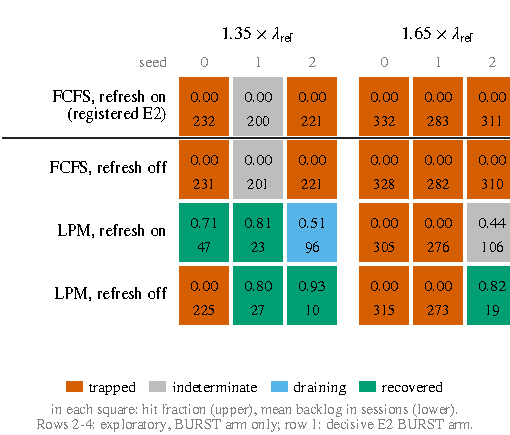
\includegraphics[width=\columnwidth]{figs/fig6_policy_grid.pdf}
\caption{Exploratory policy grid, BURST arm only, 300k pool. Rows: FCFS with the waiting-prefix refresh (the registered runs), FCFS without, LPM with, LPM without (under LPM the refresh acts only during the FCFS fallback above 128 waiting requests); below the dashed line, the exploratory vLLM 0.32.0 runs with FCFS (\S\ref{sec:vllm}), at multiples of its own $\lref$ (0.0657\sps). Columns: 1.35 and 1.65 $\lref$ by seed. Colour: registered state (RECOVERED judged on the last 300\,s); numbers: hit fraction and mean sessions in the system over the evaluation window.}\label{fig:grid}
\end{figure}

Three other engine cells ran the BURST arm at the registered rates and seeds (Fig.~\ref{fig:grid}) under exploratory registrations derived from E2's, with no control arms. In these runs the refresh made no difference for FCFS: all six runs without it, which share their arrivals with the registered runs, have the registered runs' states, hit fraction 0.000 and backlogs within 1.3\% of theirs (201--231 sessions at 1.35 $\lref$, 282--328 at 1.65), as the source predicts: the refresh moves waiting prefixes up the LRU order but does not pin them. Both rates lie inside the window; near $\lmiss$, with a cap or with the native pool, the refresh was not tested.

LPM partly helps. From the 200-session burst, at 1.35 $\lref$ it recovered in 4 of 6 runs and was draining in a fifth (hit fractions over the evaluation window; RECOVERED is judged on the last 300\,s, where every recovered run was at 0.92--0.94; with the refresh: recovered at 0.71 and 0.81, draining at 0.51; without: recovered at 0.80 and 0.93, trapped once). At 1.65 $\lref$ it was trapped in 4 of 6, indeterminate in one (hit 0.44) and recovered in one (0.82). The paths behind these window means differ from FCFS's, which had no hits from 100\,s after the burst in all twelve FCFS runs (a post-hoc reading in 100\,s windows). Each LPM run that ended trapped kept some hits until 1500--1900\,s after the burst (3900\,s in one run) and then had none; each run that recovered first exceeded a hit fraction of 0.8 3100--6500\,s after the burst and stayed above it to the end, so that had the runs ended 2000\,s earlier, only two of the five would have met the RECOVERED rule. This is a finite-burst result for the BURST arm alone, not an estimate of LPM's congested service rate $\muinf$; with mixed outcomes in every cell, three seeds do not bracket a threshold. Post hoc, the timing matches SGLang's 128-request fallback: in the five runs that recovered the engine's waiting queue never exceeded 128 after the burst, and in each of the five that ended trapped the last hit fell in the 100\,s window in which the queue last stood at or below 128. This is a correlation in ten runs, not an isolation; the exploratory LPM-INF test of \S\ref{sec:frozen} disables the fallback to test it, and Appendix~\ref{app:supp} gives the details and the other candidate causes.
